% vim: set nowrap tw=0:
\documentclass[]{llncs}
\usepackage{microtype}

% Not using NatBib but tired of fixing issues with citations being inserted in that format
\newcommand{\citep}[1]{\cite{#1}}

\usepackage{graphicx}
\usepackage{defaultstyle}
\usepackage{localstyle}
\usepackage{hanging}

\newcommand{\comment}[1]{}%\textsf{#1}}

\title{AppPAL for Android}
\subtitle{Capturing and Checking Mobile App Policies}
\titlerunning{AppPAL for Android}
% \numberofauthors{2}
\author{Joseph Hallett \and David Aspinall }
\institute{School of Informatics, University of Edinburgh}

\begin{document}

\maketitle{}

\begin{abstract}
  It can be difficult to find mobile apps that respect one's security and privacy.
  Businesses rely on employees enforcing company mobile device policies correctly.
  Users must judge apps by the information shown to them by the store.
  Studies have found that most users do not pay attention to an apps permissions during installation~\cite{Felt:2012hm} and most users do not understand how permissions relate to the capabilities of an app~\cite{Kelley:2012bw}.
  To address these problems and more, we present AppPAL: a machine-readable policy language for Android that describes precisely when apps are acceptable.
  AppPAL goes beyond existing policy enforcement tools, like Kirin~\cite{Enck:2009ko}, adding delegation relationships to allow a variety of authorities to contribute to a decision.
  AppPAL also acts as a ``glue'', allowing connection to a variety of local constraint checkers (e.g., static analysis tools, packager manager checks) to combine their results.
  As well as introducing AppPAL and some examples, we apply it to explore whether users follow certain intended policies in practice, finding privacy preferences and actual behaviour are not always aligned in the absence of a rigorous enforcement mechanism.
  \end{abstract}

\section{Introduction}
\label{sec:introduction}

Finding the right apps can be tricky.
Users need to discover which are not going to abuse their data.
This can be difficult as it isn't obvious how apps use the data each has access to.
Consider a user attempting to buy a flashlight app.
By searching the Play store the user is presented with a long list of apps.
Clicking through each one they can find the permissions each requests but not the reasons why each was needed.
They can see review scores from users but not from tools to check apps for problems and issues like SSL misconfigurations~\cite{Fahl:2012dj}.
If they want to use the app at work will it break their employers rules for mobile usage?

App stores give some information about their apps; descriptions, screenshots and review scores.
Android apps show a list of permissions when they're first installed.
In Android Marshmallow apps will display permissions requests when the app first tries to access sensitive data (such as contacts or location information).
Users do not understand how permissions relate to their device~\cite{Felt:2012hm,Thompson:2013eb}.
Ultimately the decision of which apps to use and which permissions to grant must be made by the device user.

Some apps are highly undesirable.
Many \ac{pup} are being propagated for Android devices~\cite{Truong:2014bi,Svajcer:2013tp}.
Employees are increasingly using their own phones for work.
An employer may restrict which apps their employees can use.
The IT department may set a mobile device policy---a series of rules describing what kinds of apps may be used and how---to prevent information leaks.
Some users worry that apps will misuse their personal data---sending their address book or location to an advertiser without their permission.
Such a user avoids apps which can access their location, or address book; they may apply their own personal security policies when downloading and running apps.

These policies can only be enforced by the users continuously making the correct decision when prompted about apps.
An alternative is to write the policy down and make the computer enforce it.
To implement this we propose using a logic of authorization---a language designed to express rules about permissible actions.

We present AppPAL, an instantiation of Becker~\etal's
SecPAL~\cite{Becker:2006vh} with constraints (statements checkable using information external to the language such as the time of day or static analysis tools) and predicates that allow us to decide which apps to run or install.
The language allows us to reason about apps using statements from third parties.
AppPAL allows us to enforce the policies on a device.
We can express trust relationships amongst these parties and use constraints to do additional checks, such as using security checks.
This lets us enforce more complex policies than existing tools such as Kirin~\cite{Enck:2009ko} which are limited to permissions checks.
Policies can be enforced by the stores selling the apps, on the devices installing apps or by third-parties providing app vetting services.

Consider the following example:
  a user, Alice, may have rules she has to follow when using apps for work and her own policies when using apps at home in her private life.
Using AppPAL we can write policies for work and home, and decide which policy to enforce using a user's location, or the time of day:

\noindent
\begin{minipage}{\linewidth}
  \begin{minipage}{0.5\linewidth}
    \begin{lstlisting}
'alice' says App isRunnable
  if 'home-policy' isMetBy(App)
  where at('work') = false.
    \end{lstlisting}
  \end{minipage}
  \begin{minipage}{0.5\linewidth}
    \begin{lstlisting}
'alice' says App isRunnable
  if 'work-policy' isMetBy(App)
  where beforeHourOfDay('17') = true.
    \end{lstlisting}
  \end{minipage}
\end{minipage}
\noindent We can delegate policy specification to third parties or roles, and assign principals to roles:
\begin{lstlisting}
'alice' says 'it-department' can-say 'work-policy' isMetBy(App).
'alice' says 'alice' can-act-as 'it-department'.
\end{lstlisting}
We can write policies specifying which permissions an app must or must not have by its app store categorization.
For example, it would be okay allowing a photography app access to the camera, but not to allow access to location data if the user doesn't want their photos geotagged.
\begin{lstlisting}
'alice' says App isRunnable
  if 'permissions-policy' isMetBy(App).
'alice' says 'permissions-policy' isMetBy(App)
  if App isAnApp
  where
    category(App, 'Photography'),
    hasPermission(App, 'LOCATION') = false,
    hasPermission(App, 'CAMERA') = true.
\end{lstlisting}

There has been a great amount of work on developing app analysis tools for Android.
Tools such as Stowaway~\cite{Felt:2011kj} detect over-privileged apps.
TaintDroid~\cite{Enck:2010uw} and FlowDroid~\cite{Arzt:2014kf,Li:2015wo} can do taint and control flow analysis; sometimes even between app components.
Other tools like QUIRE~\cite{Bugiel:2012ui} can find privilege escalation attacks between apps.
ScanDAL~\cite{Kim:2012vt} and SCanDroid~\cite{Fuchs:2009vi} help detect privacy leaks.
Appscopy~\cite{Feng:kPGZr_ja} searches for specific kinds of malware.
Tools like DroidRanger~\cite{Zhou:2012tb} scan app markets for malicious apps.
Various tools such as AppGuard~\cite{Backes:2012vm}, Dr.~Android~\&~Mr.~Hide~\cite{Jeon:2012ki} or AppFence~\cite{Hornyack:2011wq} can control the permissions or data an app can get.
MalloDroid~\citep{Fahl:2012dj} looks for apps configured to use SSL incorrectly (for instance by not verifying hostnames or certificates).

AppPAL can act as a \emph{``glue"} between static analysis tools and the app installation policies device owners are trying to enforce.
This avoids creating tools with hard-coded fixed policies.
 For example a store might not want to sell apps with SSL errors or apps flagged by an anti-virus tool.
Using AppPAL we can combine tools for checking apps to implement the store's policies.
\begin{lstlisting}
'play-store' says App isSellable
  if App isAnApp
  where mallodroidCheck(App) = true,
         mcafeeAVCheck(App) = true.
\end{lstlisting}
No additional attempt is made to ensure these static analysis tools are sound.
The policy designer must be aware of the tool's limitations.
Black or whitelisting may have to be used to avoid some false positives or negatives.

\section{Enforcing A Policy At Work}
\label{sec:problem}

An employee \emph{Alice} works for \emph{Emma}.
Emma allows Alice to use her personal phone as a work phone but has some specific concerns.
\begin{itemize}
  \item Alice shouldn't run any apps that can track her movements.
    Alice's workplace is at a secret location and it mustn't be leaked.
  \item Apps should come from a reputable source, such as the Google Play Store.
  \item Emma uses an \ac{av} program by McAfee.
    It should check all apps before they're installed.
\end{itemize}

To ensure this policy is met Alice promises to follow it.
She might even sign a document promising never to break the rules within the policy.
This is error-prone---what if she makes a mistake or misses an app that breaks her policy?
Alternatively Emma's policy could be partially enforced using existing tools.
\emph{Google's Device Policy for Android}~\cite{GoogleAppsDeviceP:tz} could configure Alice's device to disallow apps from outside the Google Play Store and let Emma set the permissions granted to each app~\cite{AndroidMPermission:2015uq}.

We could implement Emma's policy using existing tools (such as an AV checker, and a taint analysis tool like Flowdroid~\cite{Arzt:2014kf,Li:2015wo}) but it is a clumsy solution---they are not flexible.
Each has to be configured separately to implement only part of the policy.
If Emma changes her policy or Alice changes jobs she must recheck her apps and then alter or remove the software on her phone to ensure compliance.
It isn't clear what an app must do to be run, or what checks have been done if it is already running on the phone.
The relationship between Alice (the user), Emma (the policy setter) and the tools Emma trusts to implement her policy isn't immediately apparent.

What happens when Alice goes home?
Emma shouldn't be able to overly control what Alice does in her private life.
Alice might not be allowed to use location tracking apps at work but at home she might want to (to meet friends, track jogging routes or find restaurants for example).
Some mobile OSs, such as iOS and the latest version of Android, allow app permissions to be enabled and disabled at run time.
Can we enforce different policies at different times or locations?

% Our research looks at the problem of picking software.
% Given there are some apps you want to install and run and others you do not:
%   how can you express your preferences in such a way that they can be enforced automatically?
% How can we translate policy documents from natural language into a machine checkable form?
% How can we show the trust relationships used to make these decisions clearly and precisely?

\begin{figure}
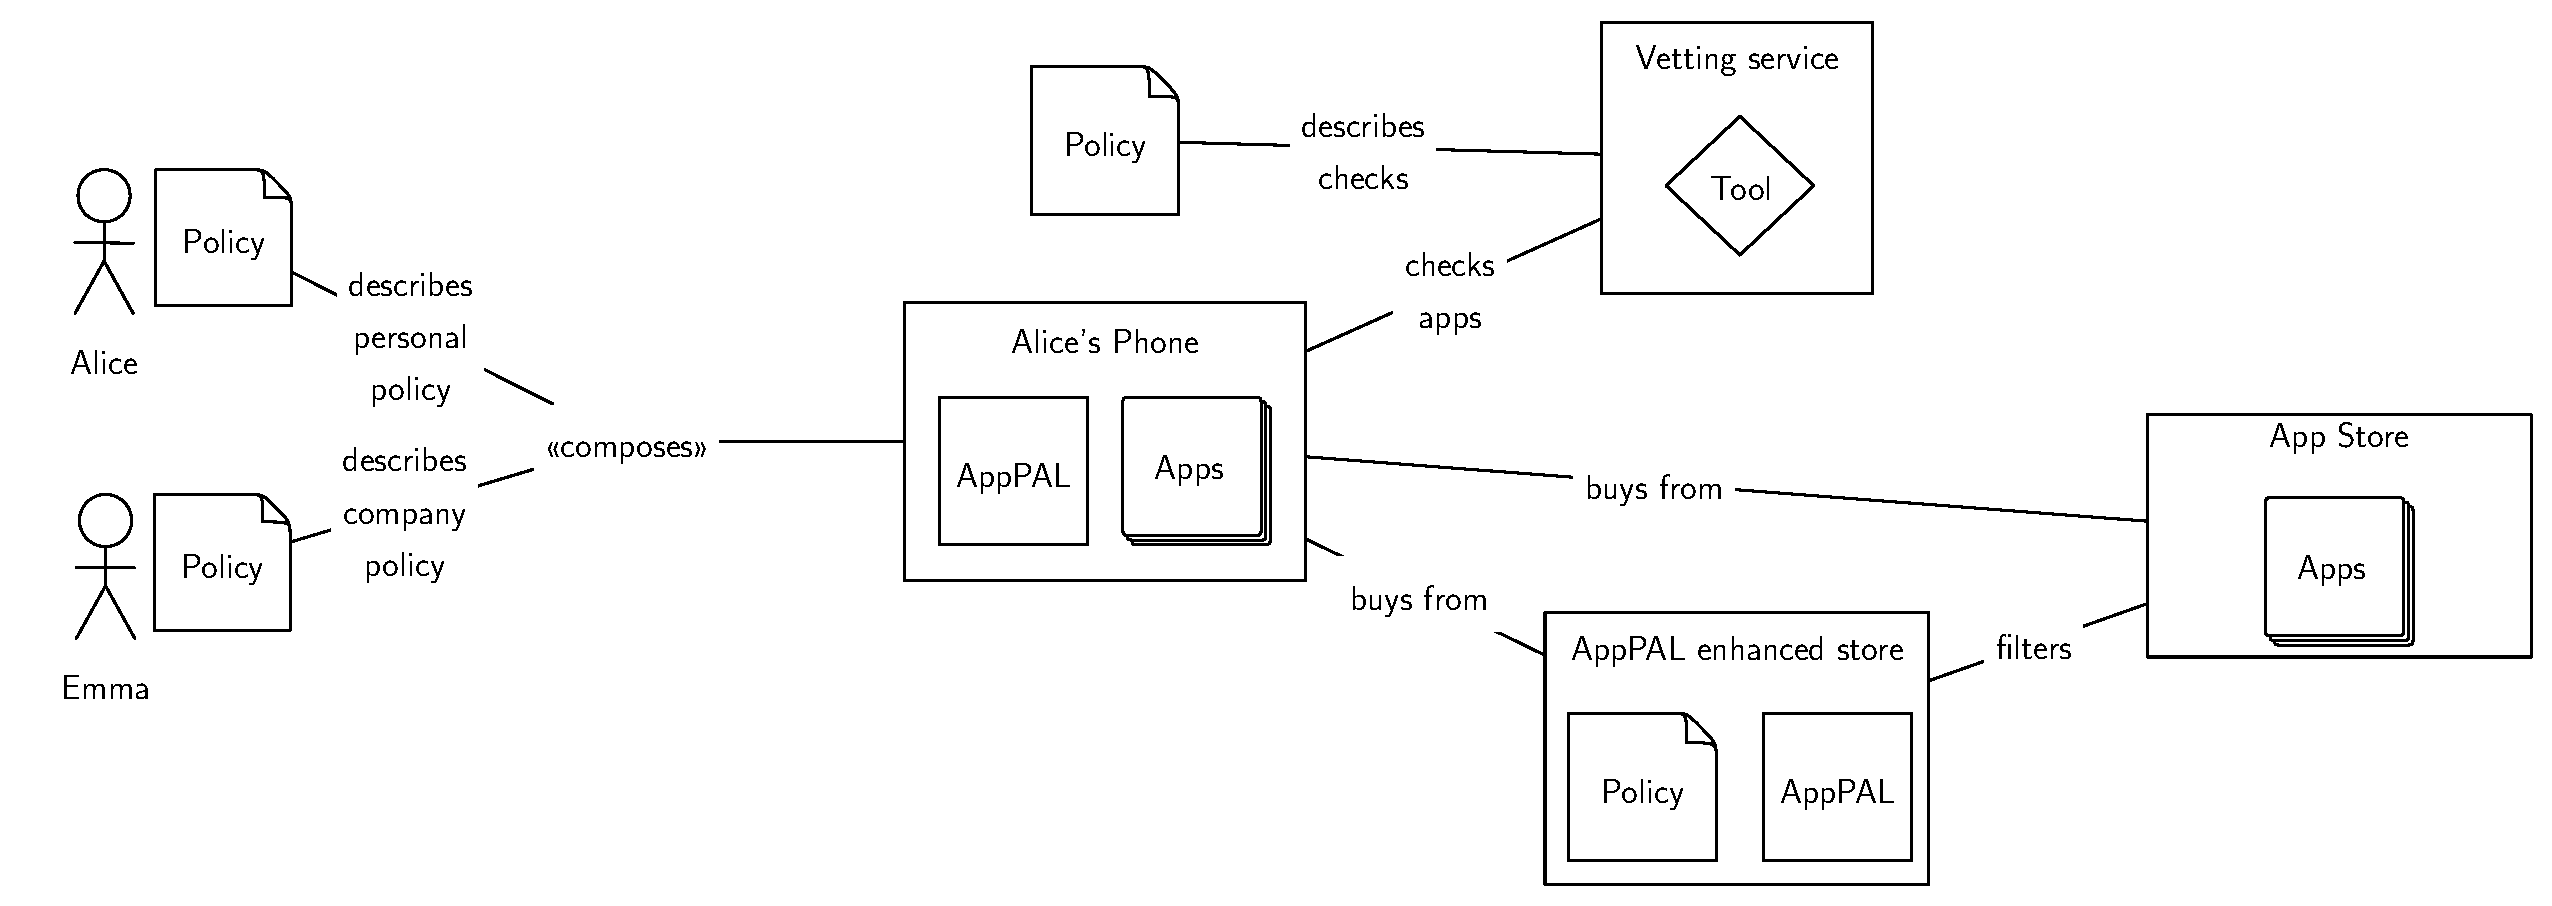
\includegraphics{figures/overview.eps}
\caption{Ecosystem of devices and stores with AppPAL.}
\label{fig:ecosystem}
\end{figure}

We propose using the mobile ecosystem shown in \autoref{fig:ecosystem}.
People have policies which are enforced by AppPAL on their devices.
They can be composed with policies from employers or others to create enhanced devices that ensure apps meet the policies of their owners.
The device can make use of vetting services which run tools to infer complex properties about apps.
Users can buy from enhanced stores which ensure the only apps they sell are the apps which meet the store's explicit policies, or ones requested by users.
Developers could decide which stores to sell their apps in on the basis of policies about stores.

\section{Expressing Policies In AppPAL}
\label{sec:idea}

In \autoref{sec:problem}, Alice and Emma had policies they wanted to enforce but no means to do so.
Instead of using several tools to enforce Emma's policy disjointedly, we could use an authorization logic.
In \autoref{lst:corporate} we give an AppPAL policy implementing Emma's app concerns on Alice's phone.
% A pictorial representation, is given in \autoref{fig:emmas_policy}; color splits statements by each speaker.

SecPAL is a logic of authorization for access control decisions in distributed systems.
It has a clear and readable syntax, as well as rich mechanisms for delegation and constraints.
SecPAL has already been used as a basis for other policy languages in areas such as privacy preferences~\cite{Becker:2009ula} and data-sharing~\cite{Aziz:2011vt}.
We present AppPAL as a modified form of SecPAL, aimed at mobile apps.

Other access control languages, such as XACML~\cite{Oasis:1M71_oFS}, could also have been used as the basis for AppPAL.
We chose to use SecPAL as the basis, however, as it was more lightweight, designed to be readable, and simpler to extend with additional constraints than XACML.

\begin{figure}
  \begin{minipage}[t]{0.44\textwidth}
    \begin{lstlisting}[numbers=left,
                       escapeinside={@}{@},
                       basicstyle=\scriptsize\ttfamily,
                       stringstyle=\scriptsize\sffamily,
                       keywordstyle=\scriptsize\slshape]
'alice' says 'emma' can-say inf
  App isRunnable. @\label{lst:corporate_1}@

'emma' says App isRunnable @\label{lst:corporate_2}@
  if 'no-tracking-policy' isMetBy(App),
     'reputable-policy' isMetBy(App),
     'anti-virus-policy' isMetBy(App).

'emma' says
  'reputable-policy' isMetBy(App) @\label{lst:corporate_3}@
      if App isBuyable.

'emma' says 'google-play' can-say
  App isBuyable. @\label{lst:corporate_4}@
    \end{lstlisting}
  \end{minipage}\begin{minipage}[t]{0.56\textwidth}
    \begin{lstlisting}[numbers=left,
                       escapeinside={@}{@},
                       firstnumber=15,
                       basicstyle=\scriptsize\ttfamily,
                       stringstyle=\scriptsize\sffamily,
                       keywordstyle=\scriptsize\slshape]
'emma' says 'anti-virus-policy' isMetBy(App) @\label{lst:corporate_5}@
  if App isAnApp
  where
    mcafeeAVCheck(App) = true.

'emma' says 'no-location-permissions'
  can-act-as 'no-tracking-policy'. @\label{lst:corporate_6}@

'emma' says
  'no-location-permissions' isMetBy(App) @\label{lst:corporate_7}@
    if App isAnApp
    where
      hasPermission(App, 'COARSE_LOCATION')=false,
      hasPermission(App, 'FINE_LOCATION')=false.
\end{lstlisting}
\end{minipage}
\caption{AppPAL policy implementing Emma's security requirements.}
\label{lst:corporate}
\end{figure}

In \autoref{lst:corporate_1} Alice lets Emma specify whether an \code{App} (a variable) \code{isRunnable};
she allows her to delegate the decision (\code{can-say}\/~\code{inf}).
Emma specifies her concerns as policies to be met in \autoref{lst:corporate_2}:
  if Emma is convinced that these are met then she will say the \code{App isRunnable}.
In \autoref{lst:corporate_3} and \autoref{lst:corporate_4} Emma specifies that an app meets the \code{reputable-policy} if the \code{App isBuyable};
  with \code{"google-play"} deciding of what is buyable or not.
Google is not allowed to delegate the decision further, i.e.~Google is not allowed to specify Amazon as a supplier of apps as well.
Emma specifies the \code{"anti-virus-policy"} in \autoref{lst:corporate_5} using a constraint.
When checking the policy the \code{mcAfeeVirusCheck} should be run on the \code{App}.
Only if this returns \code{false} will the policy be met.
To specify the \code{"no-tracking-policy"} Emma says that the \code{'no-location-permissions'} rules implement the \code{'no-tracking-policy'} (\autoref{lst:corporate_6}).
Emma specifies this in \autoref{lst:corporate_7} by checking the app is missing two permissions.

Alice wants to install a new app (\code{com.facebook.katana}) on her phone.
She collects statements to show the app meets the \code{isRunnable} predicate.
\begin{itemize}
  \item\code{"google-play" says "com.facebook.katana" isReputable.}
    Required to convince Emma that the app came from a reputable source.
  \item\code{"emma" says "anti-virus-policy" isMetBy("com.facebook.katana").}
    She can obtain this by running the \ac{av} program on her app.
  \item\code{"emma" says "no-locations-permissions" isMetBy("com.facebook.katana").}
    Needed to show the App meets Emma's no-tracking-policy.
    Emma will say this if the app has no location permissions.
\end{itemize}
These last two statements require the checker to do some extra checks to satisfy the constraints.
To get the second statement AppPAL must run the \ac{av} program on her app and check the result.
The results from the \ac{av} program may change with time as its signatures are updated;
  so the checker must re-run this check every time it wants to obtain the statement connected to the constraint.
For the third statement the AppPAL checker needs to examine the permissions of the app.
It could do this by looking in the \texttt{MANIFEST.xml} inside the app itself, or through the Android package manager if it is running on a device.

We could also imagine Emma wanting a personalised app store where all apps sold meet her policy.
With AppPAL this can be implemented by taking an existing store and selectively offering only the apps which will meet the user's policy.
This gives us a \emph{filtered store} which, from an existing set of apps, we get a personalised store that only sells apps that meet a policy.

\section{AppPAL}
\label{sec:details}
\label{ssec:language}

AppPAL is implemented as a library for Android and Java.
The parser is implemented using ANTLR4.
AppPAL's syntax is inherited from SecPAL~\cite{Becker:2006vh} (shown in \autoref{fig:assertion}).

\begin{figure}
  \newcommand{\bracetext}[1]{\text{\sffamily #1}}
  \newcommand{\smalltext}[1]{\text{\ttfamily\scriptsize #1}}
  \centering
  \begin{minipage}{0.49\linewidth}
    \begin{equation*}\small
      \begin{array}{r l}\footnotesize
        \overbrace{\smalltext{`user'}}^{\bracetext{speaker}} &
        \smalltext{ says }\overbrace{\overbrace{\smalltext{ App }}^{\bracetext{subject}}\overbrace{\smalltext{ isRunnable}}^{\bracetext{predicate}}}^{\bracetext{fact}} \\
        & \overbrace{\smalltext{ if App isFree}}^{\bracetext{condition}} \\
        & \overbrace{\smalltext{ where hasPermission(App, `INTERNET') = true}}^{\bracetext{constraint}}.
      \end{array}
    \end{equation*}
  \end{minipage}
  \begin{minipage}{0.49\linewidth}
  \newcommand{\nonterminal}[1]{$\langle$#1$\rangle$}
  \newcommand{\terminal}[1]{\textbf{#1}}
  \begin{tabular}{r c l}
    \footnotesize
    \nonterminal{Assertion} & $\coloneqq$ & \nonterminal{E} \terminal{says} \nonterminal{Fact} \\
                            &             & \hspace{1em}(\terminal{if} (\nonterminal{Fact}\terminal{,})+)?\terminal{.} \\
                            &             & \hspace{1em}(\terminal{where} \nonterminal{Constraint})? \\
    \nonterminal{Fact}      & $\coloneqq$ & \nonterminal{E} (\terminal{isRunable} $\vert$ $\ldots$) \\
                            & $\vert$     & \nonterminal{E} \terminal{can-say} \terminal{inf}? \nonterminal{Fact} \\
                            & $\vert$     & \nonterminal{E} \terminal{can-act-as} \nonterminal{E} \\
    \nonterminal{E}         & $\coloneqq$ & \terminal{Variable} $\vert$ \terminal{`constant'}
  \end{tabular}
  \end{minipage}
  \caption{Structure and simplified grammar of an AppPAL assertion.}
  \label{fig:assertion}
\end{figure}

In SecPAL the precise nature of predicates and constraints is left open.
In instantiating SecPAL, AppPAL makes the predicates and constraints explicit.
AppPAL policies can make use of the predicates and constraints in \autoref{tab:predicates}.
Additional predicates can be created in the policy files, however constraints must be implemented individually.
For example, on Android the \texttt{hasPermission} constraint uses the Android package manager to check what permissions an app requests, but the Java version uses the Android platform tools to check.

\begin{table}
  \footnotesize
  \newcommand{\style}[1]{{\footnotesize #1}}
  \begin{tabulary}{\linewidth}{l L}
  \toprule
  \style{Name}                                             & \style{Description}                                                                                                                        \\
  \midrule
  \style{App \texttt{isRunnable}}                          & \style{Says an app can be run.}                                                                                                            \\
  \style{App \texttt{isInstallable}                      } & \style{Says an app can be installed.                                                                                                     } \\
  \style{App \texttt{isAnApp}                            } & \style{Tells AppPAL that an app exists.                                                                                                  } \\
  \style{Policy \texttt{isMetBy(}App\texttt{)}           } & \style{Used to split policies into smaller components.}                                                                                    \\
  \style{\texttt{hasPermission(}App, Permission\texttt{)}} & \style{Constraint to check if an app has a permission.                                                                                   } \\
  \style{\texttt{beforeHourOfDay(}time\texttt{)}         } & \style{Constraint used to check the time.                                                                                                } \\
  \style{Tool\texttt{Check(}App, Property)               } & \style{Constraint to run an analysis tool on an app.                                                                        }              \\
  \bottomrule \\
\end{tabulary}
\caption{AppPAL predicates and constraints.}
\label{tab:predicates}
\end{table}

Splitting the decision about whether an app is runnable into a series of policies that must be met gives us flexibility in how the decision is made.
It allows us to describe multiple means of making the same decision, and provide backup routes when one fails.
Some static analysis tools are not quick to run.
Even taking minutes to run a battery draining analysis can be undesirable:
if a user wants to download an app quickly they may not be willing to wait to check that a policy is met.
In that case, it may be preferable to delegate to an online database.

In \autoref{sec:problem} and \autoref{sec:idea} we described a \emph{no-tracking-policy} to prevent a user's location being leaked.
In Emma's policy we checked this using the app's permissions;
if the app couldn't get access to the GPS sensors (using the permissions) then it meets this policy.
Some apps may want to access this data, but may not leak it.
We could use a taint analysis tool to detect this (e.g.~FlowDroid~\cite{Arzt:2014kf,Li:2015wo}).
Our policy becomes:

\begin{lstlisting}
'emma' says 'no-locations-permissions'
  can-act-as 'no-tracking-policy'.

'emma' says 'no-locations-permissions' isMetBy(App)
  if App isAnApp
  where
    hasPermission(App, 'ACCESS_FINE_LOCATION') = false,
    hasPermission(App, 'ACCESS_COARSE_LOCATION') = false.

'emma' says 'location-taint-analysis'
  can-act-as 'no-tracking-policy'.

'emma' says 'location-taint-analysis' isMetBy(App)
  if App isAnApp
  where
    flowDroidCheck(App, 'Location', 'Internet') = false.
\end{lstlisting}

Sometimes we might want to use location data.
For instance Emma might want to check that Alice is at her office.
Emma might track Alice using a location tracking app.
Provided the app only talks to Emma, and it uses SSL correctly (using MalloDroid~\cite{Fahl:2012dj}) she is happy to relax the policy.

\begin{lstlisting}
'emma' says 'relaxed-no-tracking-policy' canActAs 'no-tracking-policy'.
'emma' says 'relaxed-no-tracking-policy' isMetBy(App)
  if App hasCategory('tracking')
  where
    mallodroidSSLCheck(App) = false,
    connectionsCheck(App, '[https://emma.com]') = true.
\end{lstlisting}

This gives us four different ways of satisfying the \emph{no-tracking-policy}:
  with permissions,
  with taint analysis,
  with a relaxed version of the policy,
  or by Emma directly saying the app meets it.
When we come to check the policy if any of these ways give us a positive result we can stop our search.


\subsection{Policy Checking}
\label{ssec:eval}

AppPAL has the same policy checking rules as SecPAL~\cite{Becker:2006vh}.
AppPAL uses an assertion context of known facts and rules, as well as facts deduced while checking.
While Becker~\etal~used a DatalogC based checking algorithm, we have implemented the rules directly in Java as no DatalogC library is currently available for Android.
Pseudo-code is shown in \autoref{fig:pseudocode}.

On a mobile device memory is at a premium.
We want to keep the assertion context as small as possible.
For some assertions (like \code{isAnApp}) we derive them by checking the arguments at evaluation time.
This gives us greater control of the evaluation and how the assertion context is created.
For example, when checking the \code{isAnApp} predicate;
  we can fetch the assertion that the subject is an app based on the app in question.
When delegating we will also be able to request facts from the delegated party dynamically (although this is not yet implemented).

\begin{figure}\centering
\begin{minipage}[b]{0.49\linewidth}
\begin{lstlisting}[language=Ruby, basicstyle=\ttfamily\scriptsize, keywordstyle=\scriptsize\slshape, columns=flexible]
def evaluate(ac, rt, q, d)
  return rt[q, d] if rt.contains q, d
  p = cond(ac, rt, q, d)
  if p.isValid then
    return (Proven, rt.update q, d, p)
  p = canSay_CanActAs(ac, rt, q, d)
  if p.isValid then
    return (Proven, rt.update q, d, p)
  else
    return (Failure, rt.update q, d, Failure)
\end{lstlisting}
\end{minipage}
\begin{minipage}[b]{0.49\linewidth}
\begin{lstlisting}[language=Ruby, basicstyle=\ttfamily\scriptsize, keywordstyle=\scriptsize\slshape, columns=flexible]
def canSay_CanActAs(ac, rt, q, d)
  ac.constants.each do |c|
    if c.is_a :subject
      p = canActAs ac, rt, q, d
      return Proven if p.isValid
    elsif c.is_a :speaker
      p = canSay ac, rt, q d
      return Proven if p.isValid
  return Failure
\end{lstlisting}
\end{minipage}

\begin{minipage}[b]{0.49\linewidth}
\begin{lstlisting}[language=Ruby, basicstyle=\ttfamily\scriptsize, keywordstyle=\scriptsize\slshape, columns=flexible]
def cond(ac, rt, q, d)
  ac.add q.fetch if q.isFetchable
  ac.assertions.each do |a|
    if (u = q.unify a.consequent) &&
       (a = u.sub a).variables == none
      return checkConditions ac, rt, a, d
  return Failure
\end{lstlisting}
\end{minipage}
\begin{minipage}[b]{0.49\linewidth}
\begin{lstlisting}[language=Ruby, basicstyle=\ttfamily\scriptsize, keywordstyle=\scriptsize\slshape, columns=flexible]
def checkConditions(ac, rt, a, d)
  getVarSubs(a,ac.constants).each do |s|
    sa = s.sub a
    if sa.antecedents.all
        { |a| evaluate(ac, rt, a, d).isValid }
      p = evaluateC sa.constraint
      return Proven if p.isValid
  return Failure
\end{lstlisting}
\end{minipage}
\caption{Partial-pseudocode for AppPAL evaluation.}
\label{fig:pseudocode}
\end{figure}

\subsection{Benchmarks}
\label{ssec:benchmarks}

When AppPAL runs on a mobile phone, apps should be checked as they are installed.
Since policy checks may involve inspecting many rules and constraints one may ask whether the checking will be acceptably fast.
Downloading and installing an app takes about 30 seconds on a typical Android phone over wifi.
If checking a policy delays this even further a user may become annoyed and disable AppPAL.

The policy checking procedure is at its slowest when having to delegate repeatedly;
   the depth of the delegation tree is the biggest factor for slowing the search.
Synthetic benchmarks were created to check that the checking procedure performed acceptably.
Each benchmark consisted of a chain of delegations.
The \emph{1 to 1} benchmark consists of a repeated delegation between all the principals.
In the \emph{1 to 2} benchmark each principal delegated to 2 others and in the \emph{1 to 3} benchmark each principal delegated to 3 others.
These benchmarks are reasonable as they model the slowest kinds of policies to
evaluate---though worse ones could be designed by delegating even more or triggering an expensive constraint check.

For each benchmark we controlled the number of principals in the policy file:
  as the number of principals increased so did the size of the policy.
The results are shown in \autoref{fig:benchmarks}.
We have only used a few delegations per decision when describing hypothetical user policies.
We believe the policy checking performance of AppPAL is acceptable as unless a policy consists of hundreds of delegating principals the overhead of checking an AppPAL policy is negligable.

\begin{figure}
  \centering
  \begin{minipage}{0.40\linewidth}
    \scriptsize
    \begin{tabular*}{0.80\linewidth}{c c r@{.}l}
      \toprule
      Delegations & Principals & \multicolumn{2}{c}{Time (s)} \\
      \midrule
      1 to 1 & 10   &  0&01 \\
      1 to 1 & 100  &  1&00 \\
      1 to 1 & 500  & 20&90 \\
      1 to 1 & 1000 & 88&73 \\
      \midrule
      1 to 2 & 10   &  0&01 \\
      1 to 2 & 100  &  0&43 \\
      1 to 2 & 500  &  7&36 \\
      1 to 2 & 1000 & 27&47 \\
      \midrule
      1 to 3 & 10   &  0&01 \\
      1 to 3 & 100  &  0&24 \\
      1 to 3 & 500  &  3&99 \\
      1 to 3 & 1000 & 15&28 \\
      \bottomrule
    \end{tabular*}
  \end{minipage}
  \begin{minipage}{0.59\linewidth}
    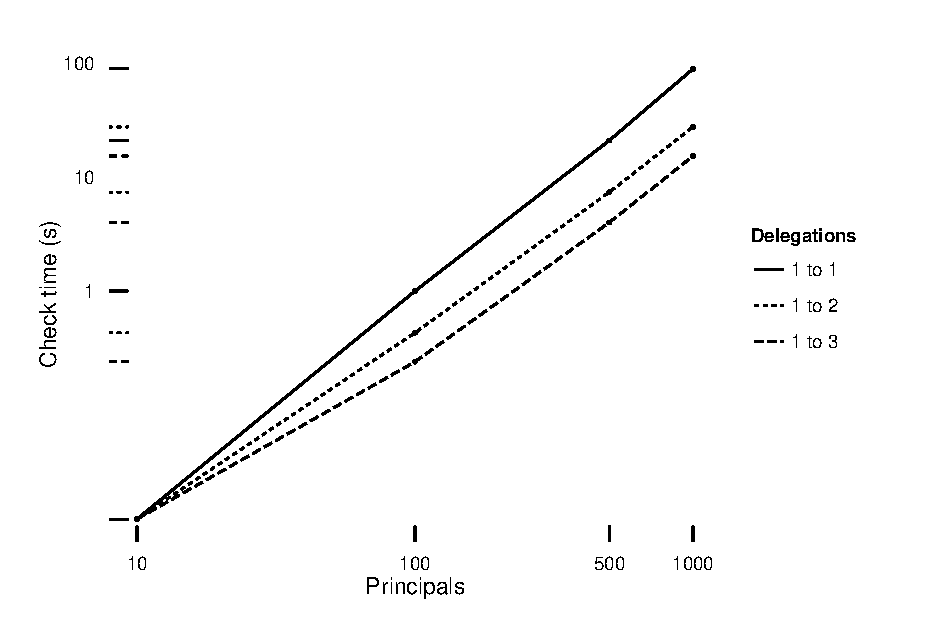
\includegraphics[width=\linewidth]{figures/benchmarks.eps}
  \end{minipage}
  \caption{Benchmarking results on a Nexus 4 Android phone.}
  \label{fig:benchmarks}
\end{figure}

\section{Measuring Policy Compliance}
\label{sec:demonstation}

Throughout we have asserted that users often have informal policies and that there is a need for policy enforcement tools.
Corporate mobile security \ac{byod} policies have started appearing and NIST have issued recommendations for writing them~\cite{Scarfone:2009vy,Souppaya:2013jf}.
In a study of 725 Android users, Lin~\etal~found four patterns that characterise user privacy preferences for apps~\cite{Sadeh:2014vq} demonstrating a refinement of Westin's privacy segmentation index~\cite{Krane:2002jo}.
Using app installation data from Carat~\cite{Oliner:2013ht,Chia:2012gz} we used AppPAL to find the apps satisfying each policy Lin~\etal~identify and measure the extent that each user was following a policy.

Lin~\etal~identified four types of user.
The \emph{Conservative} (C) users were uncomfortable allowing an app access to any personal data for any reason.
The \emph{Unconcerned} (U) users felt okay allowing access to most data for almost any reason.
The \emph{Advanced} (A) users were comfortable allowing apps access to location data but not if it was for advertising.
Opinions in the largest cluster, \emph{Fencesitters} (F), varied but were broadly against collection of personal data for advertising.
We wrote AppPAL policies to describe each of these behaviours as increasing sets of permissions.
These simplify the privacy policies identified by Lin~\etal~as we do not take into account the reason each app might have been collecting each permission
(we could write more precise rules if we could determine why each permission was requested).
Lin~\etal~used Androguard~\cite{Desnos:ub} as well as manual analysis to determine the precise reasons for each permission~\cite{Sadeh:2014vq}.

\newcommand{\tabtitle}[1]{\textbf{\footnotesize #1}}
\begin{center}
  \begin{tabular}{ r l l l l }
%                                     & \rothead{Conservative} & \rothead{Advanced} & \rothead{Fencesitter} & \rothead{Unconcerned} \\
    \toprule
    \tabtitle{Policy}                 & \tabtitle{C}           & \tabtitle{A}       & \tabtitle{F}          & \tabtitle{U}          \\
    \midrule
    \texttt{GET\_ACCOUNTS}            & \xmark                 & \xmark             & \xmark                & \xmark                \\
    \texttt{ACCESS\_FINE\_LOCATION}   & \xmark                 & \xmark             & \xmark                &                       \\
    \texttt{READ\_CONTACT}            & \xmark                 & \xmark             & \xmark                &                       \\
    \texttt{READ\_PHONE\_STATE}       & \xmark                 & \xmark             &                       &                       \\
    \texttt{SEND\_SMS}                & \xmark                 & \xmark             &                       &                       \\
    \texttt{ACCESS\_COARSE\_LOCATION} & \xmark                 &                    &                       &                       \\
    \bottomrule
  \end{tabular}
\end{center}

It is also interesting to discover when people install apps classified as malware.
McAfee classify malware into several categories, and provided us with a dataset of apps classified as malware and \ac{pup}s.
The \emph{malicious} and \emph{trojan} categories describe traditional malware.
Other categories classify \ac{pup} such as aggressive adware.
Using AppPAL we can write policies to differentiate characterising users who allow dangerous apps and those who install poor quality ones.
\begin{lstlisting}
'user' says 'mcafee' can-say
  'malware' isKindOf(App).
'mcafee' says 'trojan' can-act-as 'malware'.
'mcafee' says 'pup' can-act-as 'malware'.
\end{lstlisting}
If a user is enforcing a privacy policy we might also expect them to install less malware.
We can check this by using AppPAL policies to measure the number of malwares each user had installed.

We now want to test how closely user behavior follows policies.
Installation data was taken from a partially anonymized\footnote{Users are replaced with incrementing numbers, app names are replaced with hashes to protect sensitive names.} database of installed apps captured by Carat~\cite{Oliner:2013ht}.
By calculating the hashes of known package names we see who installed what.
The initial database has over 90,000 apps and 55,000 users.
On average each Carat user installed around 90 apps each; 4,300 apps have known names.
Disregarding system apps (such as \texttt{com.android.vending}) and very common apps (Facebook, Dropbox, Whatsapp, and Twitter) we reduced the set to an average of 20 known apps per user.
To see some variation in app type, we considered only the 44,000 users who had more than 20 known apps.
Using this data, and the apps themselves taken from the Google Play Store and Android Observatory~\cite{Barrera:2012iba}, we checked which apps satisfied which policies.

\begin{figure}\centering
  \subfigure[Uptake of Lin~\etal's policies.]{%
    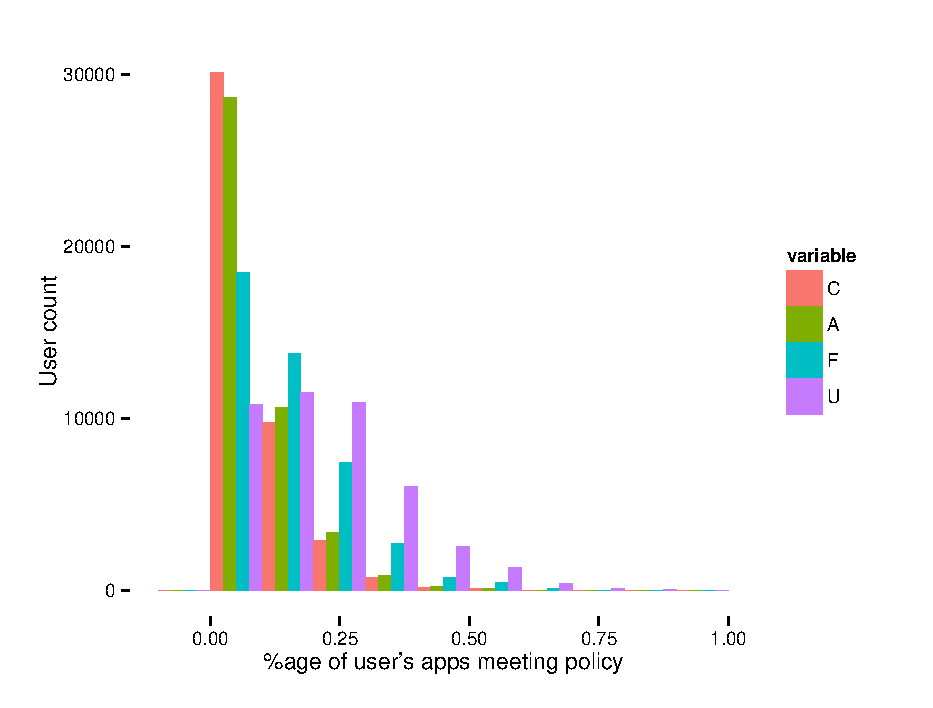
\includegraphics[width=0.48\linewidth]{./figures/lin.eps}
    \label{fig:lin}}
  \subfigure[Uptake of malware and PUPs.]{%
    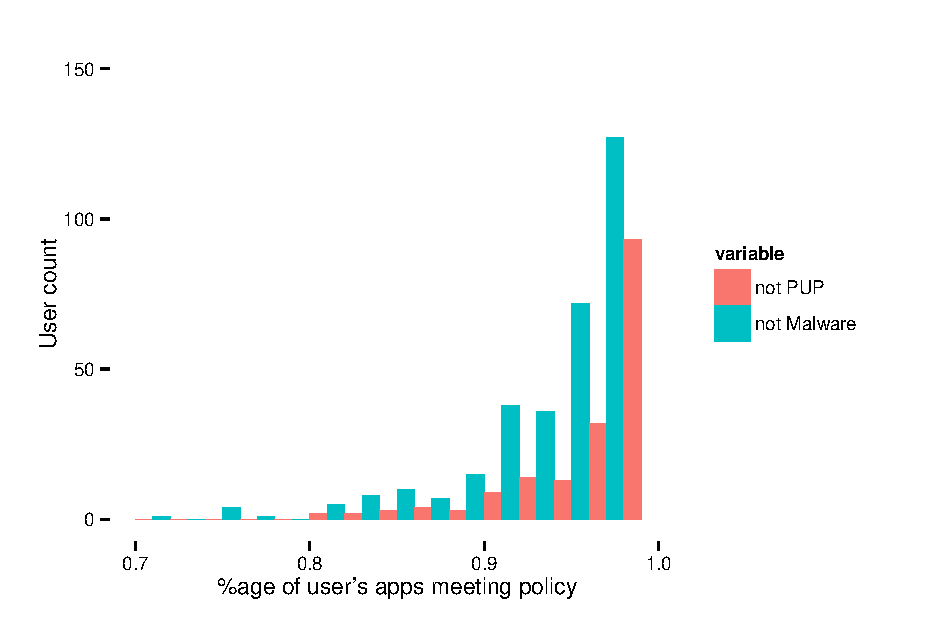
\includegraphics[width=0.48\linewidth]{./figures/malware.eps}
    \label{fig:malware}}
    \caption{Policy compliance graphs. Each histogram shows the number of users who followed a policy to a certain extent.  Users who installed no malware have been omitted from Figure~\autoref{fig:malware}.}
\end{figure}

Figure~\ref{fig:lin} shows that very few users follow Lin~\etal's policies most of the time.
Whilst the AppPAL policy we used was a simplified version of Lin~\etal's policy, it suggests that there is a disconnect between user's privacy preferences and their behaviour (reminiscent of the \emph{privacy paradox}); assuming the user population studied by Lin~\etal~behave similarly to data from the Carat study.
A few users, however, did seem to be installing apps meeting these policies most of the time.
This suggests that while users may have privacy preferences the majority are not attempting to enforce them.
Policy enforcement tools, like AppPAL, can help users enforce their own policies which they cannot do easily using the current ad hoc, manual  means available to them.

\begin{figure}\centering
  \subfigure[Advanced and non-\ac{pup} policies.]{%
    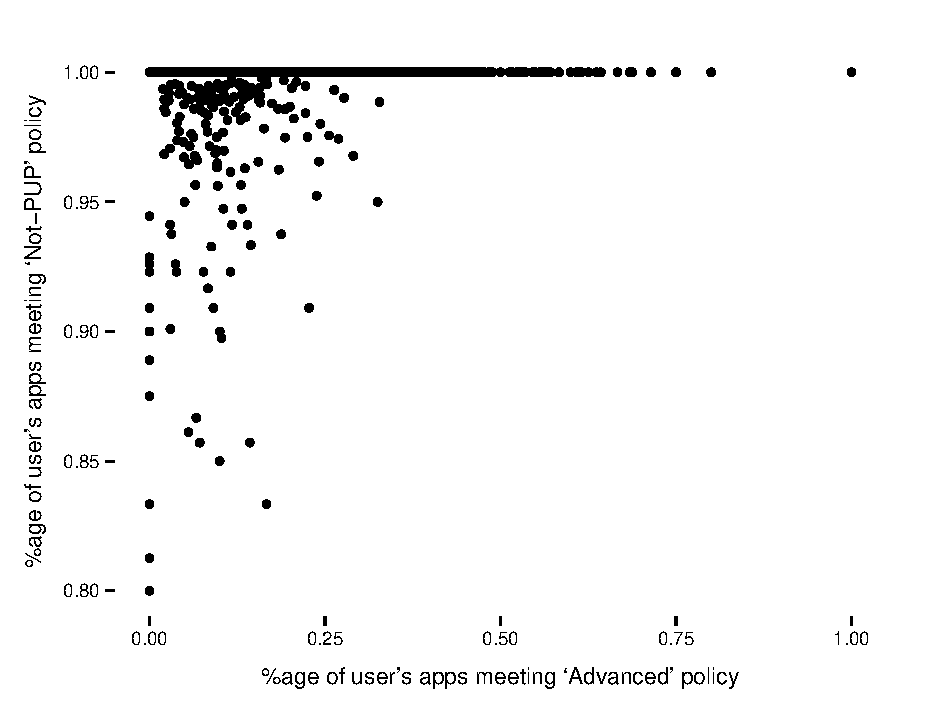
\includegraphics[width=0.48\linewidth]{./figures/advanced-v-pup.eps}
    \label{fig:versus_pup}}
    \subfigure[Advanced and SSL policies.]{%
    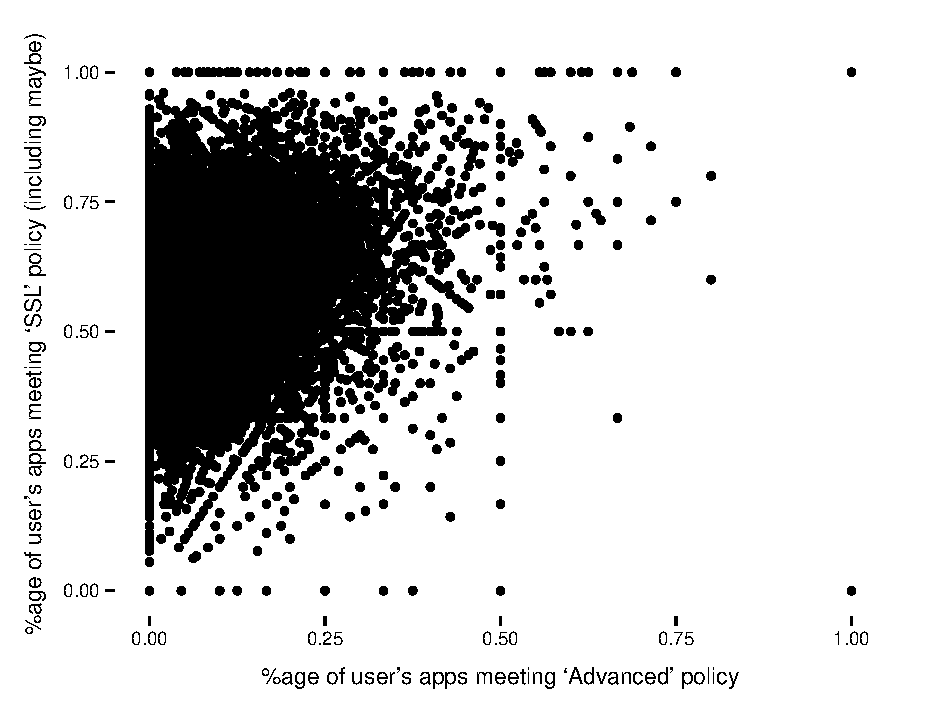
\includegraphics[width=0.48\linewidth]{./figures/advanced-v-mallodroid_m.eps}
    \label{fig:versus_mallodroid}}
    \caption{Compliance with the advanced policy and the non-\ac{pup} and SSL policies.  Each data-point represents a user.  In (a) we see that users who followed the Advanced policy more than 50\% of the time did not install any malware.  In (b) we see that even users who followed the Advanced policy were no better at avoiding apps with SSL problems than any other users.}
  \label{fig:versus}
\end{figure}

We found that 1\% of the users had a \ac{pup} or malicious app installed.
Figure~\ref{fig:malware} shows that infection rates for \ac{pup}s and malware is low;
though a user is 3 times more likely to have a \ac{pup} installed than malware.
Users who were complying more than half the time with the conservative or advanced policies complied with the malware or \ac{pup} policies fully (Figure~\autoref{fig:versus_pup}).
This suggests that policy enforcement is worthwhile: users who can enforce policies about their apps experience less malware.

The \emph{MalloDroid} tool~\citep{Fahl:2012dj} can scan apps for SSL misconfigurations.
SSL misconfigurations are dangerous as they can undermine any privacy guarantees that SSL/TLS gives.
MalloDroid distinguishes cases where the app is definitely misconfigured from those where there is some doubt.
We set up AppPAL to use MalloDroid results as a constraint and measured the percentage of apps each Carat user had installed that did not have issues or suspected issues when scanned with MalloDroid.
Users who were complied with the advanced policy were no better at avoiding apps with SSL errors than any other users, see Figure~\autoref{fig:versus_mallodroid}.
This emphasizes that AppPAL can help enforce complex policies that cannot be checked without additional tools.

There are limitations in this study:
first, we do not have the full user purchase history, and we can only find out about apps whose names match those in available databases.
So a user may have apps installed that break the policy without us knowing.
Second, recently downloaded apps used for experiment may not be the same version that users had, in particular, their permissions may differ.
Permissions tend to increase in apps over time~\cite{Wei:2012id}; so a user may be more conservative than our analysis suggests.
Finally, as mentioned, we have compared a different set of users to the ones Lin~\etal~looked at.
We plan to do a more comprehensive user study in the future that investigates AppPAL in use with different communities.

\section{Related Work}

Authorization logics have been used to enforce policies in several other domains.
The earliest such logic, PolicyMaker~\cite{Blaze:dj}, was general and undecidable.
Logics that followed like KeyNote~\cite{Blaze:1999fa} and SPKI/SDSI~\cite{Ellison:1999ui} looked at public key infrastructure.
The RT-languages~\cite{Li:2002if} were designed for credential management.
Cassandra~\cite{Becker:2004fi} was used to model trust relationships in the British national health service.

SELinux is used to describe policies for Linux processes, and for access control (on top of the Linux discretionary controls).
It was ported to Android~\cite{Smalley:2013vl} and is used in the implementation of the permissions system.
SELinux describes the capabilities (in terms of system calls and file access) of processes, it cannot describe app installation policies or delegation relationships.
Google also offer the \emph{Device Policy for Android} app.
This lets businesses configure company-owned devices to be trackable, remote lockable, set passwords and sync with their servers.
It cannot be used to describe policies about apps, or describe trust relationships.

The SecPAL language is designed for access control in distributed systems.
We picked SecPAL as the basis for AppPAL because it is readable, extensible, and is a good fit for the mobile ecosystem setting~\citep{Hallett:2014un}.
It has also been used to describe data usage policies~\cite{Aziz:2011vt} and inside Grid data systems~\cite{Humphrey:2007wc}.
Other work has added various features such as existential
quantification~\cite{Becker:2009vt} and extended to the DKAL family of languages~\cite{Gurevich:2008fz,Gurevich:Qo5E3M3}.
DKAL contains more modalities than \emph{says}, which lets policies describe actions principals carry out rather than just their opinions.
For example in AppPAL a user might \emph{say} an app is installable if they would install it (\code{"user" says App isInstallable}).
In DKAL they can describe the conditions that would force them to install it (\code{"user" installs App}).
With DKAL we can guarantee that the action was completed, whereas in AppPAL we do not know if the user actually installed a particular app.
We chose to use SecPAL as the basis for AppPAL as we did not need the extra features DKAL added to express app installation policies for our initial applications.

Kirin~\cite{Enck:2009ko} is a policy language and tool for enforcing app installation policies to prevent malware.
Policy authors can specify combinations of permissions and broadcast events that should not appear together.
For example, to stop malware sending premium rate text messages, we prevent an app having both the \texttt{SEND\_SMS} and \texttt{WRITE\_SMS} permissions:

\lstinline!restrict permission [SEND_SMS] and permission [WRITE_SMS]!

By analyzing apps which broke their policies Enck~\etal~found vulnerabilities in Android, but were ultimately limited by being restricted to permissions and broadcast events.

The Kirin approach has been shown to help identify malware, but it is less suitable for detecting \acp{pup}.
The behaviours and permissions \ac{pup} displays aren't necessarily malicious.
One user may not want apps which need in-app-purchases to play, but another may enjoy them.
With Kirin we are restricted to permitting or allowing apps.
AppPAL can describe more scenarios than just allow or forbid, and use more app information than just permissions, such as constraints and static analysis results.
By allowing delegation relationships we can understand the provenance and trust relationships in these rules.

\section{Conclusions and Further Work}

We have presented AppPAL: a language for describing app installation policies to help achieve security and privacy objectives but which can also \emph{lock down} devices in other ways, e{.}g{.}~restricting the use of certain apps while at work.
We showed how static analysis tools can be connected to AppPAL to compose complex properties.

Further work is needed to tightly integrate AppPAL into Android.
One way to integrate AppPAL on Android would be as a \emph{required checker}: a program that checks all apps before installation.
Google uses the required checker API to check for known malware and jailbreak apps.
We would use AppPAL to check apps meet policies before installation.
The API is protected, however, and it would require the phone to have a custom firmware.
This is undesirable as it would make AppPAL difficult to install for most users, and negate the other security enhancements (such as timely updates and patches) provided by the standard Android system.
AppPAL could be integrated as a service to reconfigure app permissions.
Android Marshmallow has an iOS like permissions model where permissions can be granted and revoked at any time.
These will be manually configurable by the user through the settings app.
We can imagine AppPAL working to reconfigure these settings (and set the device's initial grant or deny states) based on a user's policy, as well as the time of day or the user's location.
A policy could deny notifications while a user is driving, for example, by checking if they are using Android Auto~\cite{AndroidAuto:uw} (an app to interact with a car's center console) or moving along a road at high speed.

Future work includes developing and testing, policies for users.
Here we described a policy being specified by a user's employer.
For most end-users writing a policy in a formal language unrealistic.
With Ad-blocking software users subscribe to filter policies written by experts, such as EasyList\footnote{\url{https://easylist.adblockplus.org/en/}}.
We can imagine a similar scheme working well for app installation policies.
Users subscribe to different policies by experts (examples could include no tracking apps, nothing with adult content, no in-app-purchase apps).
Optionally the users could customize the policies further, similar to proof-carrying code~\cite{Necula:1996tr}.

Policy composition raises further questions: what should happen when user's personal and work policies overlap?  
What should happen when policies contradict? 
Future work will look at detecting these problems as well as integrating strategies to resolve them.

Another question might be whether we can use evidence to speed re-checking apps against a policy.
Some static analysis tools, such as Evicheck~\cite{Seghir:2015er}, can create evidence that lets you check an app doesn't have certain behavior faster than it would be to infer the same property in the app without it.
We can also imagine apps being distributed with evidence that proves the app meets an AppPAL policy but avoids the need to check the against the policy explicitly.


We might attempt to learn policies from existing user's behavior.
Given app usage data, from a project like Carat~\cite{Oliner:2013ht}, we could identify security conscious users.
If we can infer these users policies we may be able to describe new policies that the less technical users may want.
Given a set of apps one user has already installed, we could learn policies about what their personal security relevant installation policy is.
This may help stores show users apps they're more likely to buy, and users apps that already behave as they want.

AppPAL gives us a framework for describing and evaluating policies for Android apps.
The work provides new, rigorous, ways for machines to enforce user's and device-owner's rules about how apps should behave.
These policies can be enforced more reliably, and with less interaction from person operating the device.

\subsection*{Acknowledgements}

Thanks to Igor~Muttik at McAfee, and N~Asokan at Aalto University and the University of Helsinki for discussions and providing us with data used in \autoref{sec:demonstation}.
Thanks also to the App Guarden project and colleagues at the University of Edinburgh for their comments, and the referees for their feedback.

\bibliographystyle{splncs03}
\bibliography{paper}
\end{document}

